
\section{Trigonometry}

Let $P$ be a point on a unit circle $x^2+y^2=1$. Let $\theta$ be the
distance from $(1,0)$ to $P$ measured counterclockwise along the
circle. Then the coordinates of $P$ are
$(\cos\theta,\sin\theta)$.\footnote{The order is easy to remember-- it's
  alphabetical.}

\begin{figure}[htbp]
  \centering
  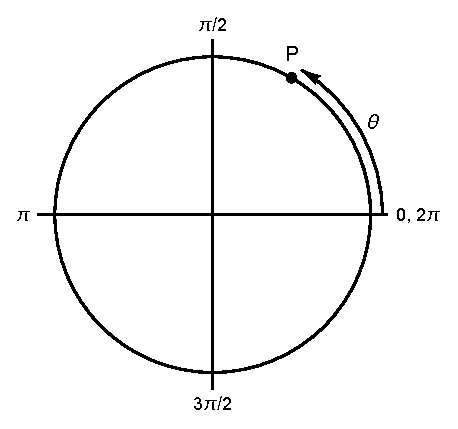
\includegraphics[width=0.5\textwidth]{trigtldr.eps}
\end{figure}

Recall the circumference of a circle is $C=2\pi r$, and so the
circumference of a unit circle is $2\pi$. Thus $\pi$ represents $180^\circ$.

%%% Local Variables:
%%% TeX-master: "precalc"
%%% End:
